\begin{figure}
  \centering
  \vspace*{-0.25cm}
  \hspace*{-0.5cm}
  \begin{tikzpicture}    
    \node at (0, 0){
      \includegraphics[width=6cm]{experiments/3d/vae_occ_aml/easy_15/results_0}
    };
    \node at (0, -4.25){
      \includegraphics[width=6cm]{experiments/3d/vae_evae/easy_15/results_0}
    };
    \node at (0, -8.75){
      \includegraphics[width=6cm]{experiments/3d/vae_evae/moderate_15/results_0}
    };
    
    %\draw[-,dashed] (3.25, -3) -- (3.25,3);
    
    \node at (6.5, 0){
      \includegraphics[width=6cm]{experiments/3d/vae_occ_aml/easy_15/results_1}
    };
    \node at (6.5, -4.25){
      \includegraphics[width=6cm]{experiments/3d/vae_evae/easy_15/results_1}
    };
    \node at (6.5, -8.75){
      \includegraphics[width=6cm]{experiments/3d/vae_evae/moderate_15/results_1}
    };
    
    \node at (10,0) {
      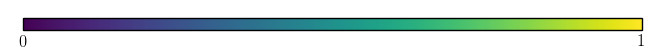
\includegraphics[height=4.25cm]{experiments/3d/vae_occ/easy_15/colorbar}
    };
   
    \draw[-,dashed] (-3.5,-2.125) -- (10,-2.125);
    \draw[-,dashed] (-3.5,-6.5) -- (10,-6.5);
    
    \node[rotate=90] at (-4, 0) {\begin{tabular}{c}\AML\\\easy\end{tabular}};
    \node[rotate=90] at (-4, -4.25) {\begin{tabular}{c}\EVAE\\\easy\end{tabular}};
    \node[rotate=90] at (-4, -8.75) {\begin{tabular}{c}\EVAE\\\moderate\end{tabular}};
    
  \end{tikzpicture}
  \vskip 2px
  
  % TODO short caption
  \caption{Qualitative results for \AML and \EVAE on occupancy only considering
  the \easy and \hard cases of the 3D cuboids dataset. As can be seen, both
  approaches perform reasonably well in these cases. As before, we show
  horizontal slices of the volumes, in particular
  heights $8 + 2i$ for $0 \leq i < 8$.}
  \label{fig:appendix-experiments-3d-aml-qual-1}
\end{figure}
\begin{figure}
  \centering
  \vskip -0.25cm
  \begin{tikzpicture}  
    \node at (0, 0){
      \includegraphics[width=6cm]{experiments/3d/vae_occ_sdf_aml/easy_15/results_0_0}
    };
    \node at (0, -4){
      \includegraphics[width=6cm]{experiments/3d/vae_occ_sdf_aml/easy_15/results_1_0}
    };
      
    \node at (0, -8.5){
      \includegraphics[width=6cm]{experiments/3d/vae_occ_sdf_aml/moderate_15/results_0_0}
    };
    \node at (0, -12.5){
      \includegraphics[width=6cm]{experiments/3d/vae_occ_sdf_aml/moderate_15/results_1_0}
    };
    
    \draw[-,dashed] (-3.5, -6.25) -- (10,-6.25);
    
    \node at (6.5, 0){
      \includegraphics[width=6cm]{experiments/3d/vae_occ_sdf_aml/easy_15/results_0_1}
    };
    \node at (6.5, -4){
      \includegraphics[width=6cm]{experiments/3d/vae_occ_sdf_aml/easy_15/results_1_1}
    };
    
    \node at (6.5, -8.5){
      \includegraphics[width=6cm]{experiments/3d/vae_occ_sdf_aml/moderate_15/results_0_1}
    };
    \node at (6.5, -12.5){
      \includegraphics[width=6cm]{experiments/3d/vae_occ_sdf_aml/moderate_15/results_1_1}
    };
    
    \node at (10,0) {
      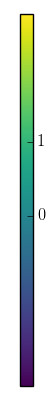
\includegraphics[height=4.25cm]{experiments/3d/vae_occ_sdf_aml/colorbar_1}
    };
    
    \node at (-3.5,0) {
      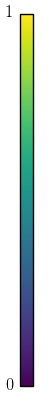
\includegraphics[height=4.25cm]{experiments/3d/vae_occ_sdf_aml/colorbar_0}
    };
    
    %\node[rotate=90] at (-3.5,-2) {\begin{tabular}{c}\AML +sdf\\\easy\end{tabular}};
    %\node[rotate=90] at (-3.5,-10.5) {\begin{tabular}{c}\AML +sdf\\\moderate\end{tabular}};
    
    \node[rotate=90] at (-3.5,-4) {\easy};
    \node[rotate=90] at (-3.5, -8.5) {\moderate};
    
    \node at (0, 2.25) {occupancy};
    \node at (6.5, 2.25) {signed distance function};
    
  \end{tikzpicture}
  \vskip 6px
  
  % TODO short caption
  \caption{Qualitative results for \AML using both occupancy and signed distance
  functions on \easy and \moderate difficulties of the 3D cuboids dataset.
  Here, \AML has considerable difficulties on \moderate difficulty. We show
  the corresponding horizontal slices of the volumes, \ie height levels
  $8 + 2i$ for $0 \leq i < 8$.}
  \label{fig:appendix-experiments-3d-aml-qual-2}
\end{figure}